%!TEX root = bipartite.tex

\section{Evaluation} \label{sec:eval}

To illustrate the proposed method for user-objects network we apply it to
Davis's Southern Women dataset \citep{davis1941deep} and the five real-world
datasets presented in section \ref{sec:ubnetworks}. First we are going to
analyse Davis's data in more detail.

\paragraph{Southern women}

\begin{figure}[t] \centering
  \begin{tabular}{c} 
  \subfloat[Tf-idf
  weights]{\label{fig:southern_tfidf}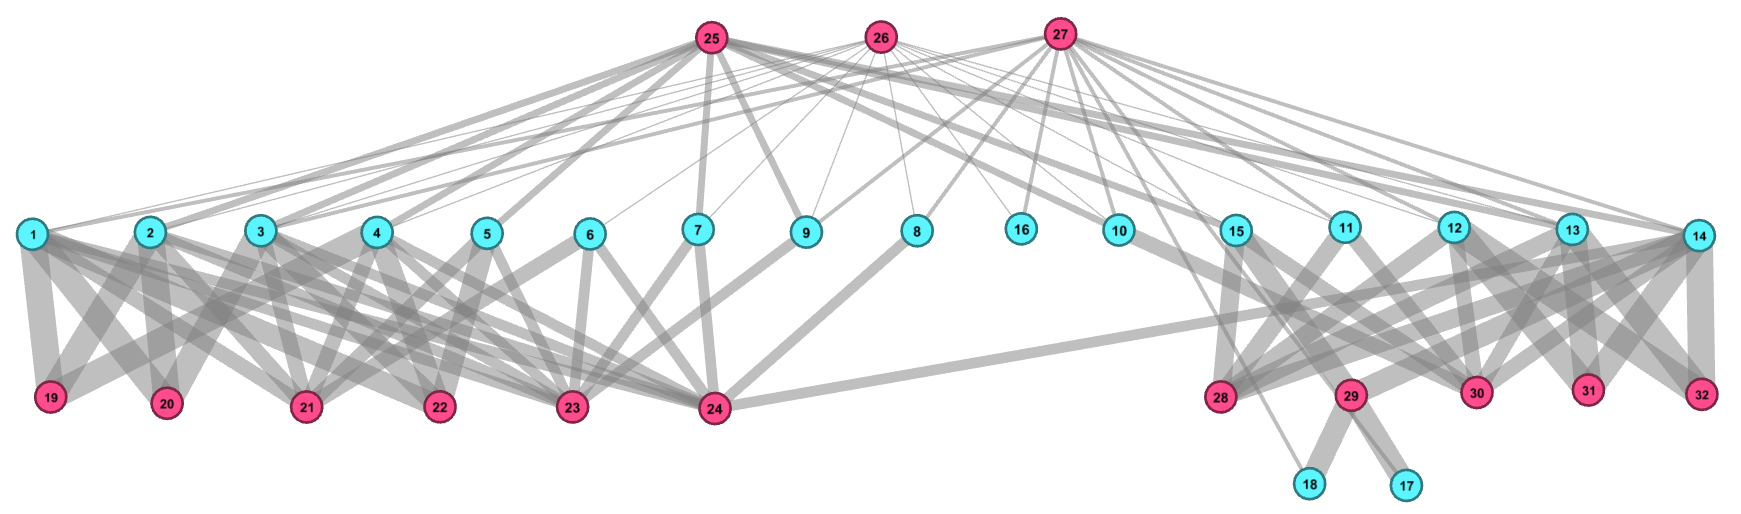
\includegraphics[width=14cm]{./figures/southern_tfidf.png}}
  \\   
      \subfloat[Filtered
      network
      $\tau
      =
      1$]{\label{fig:southern_rm}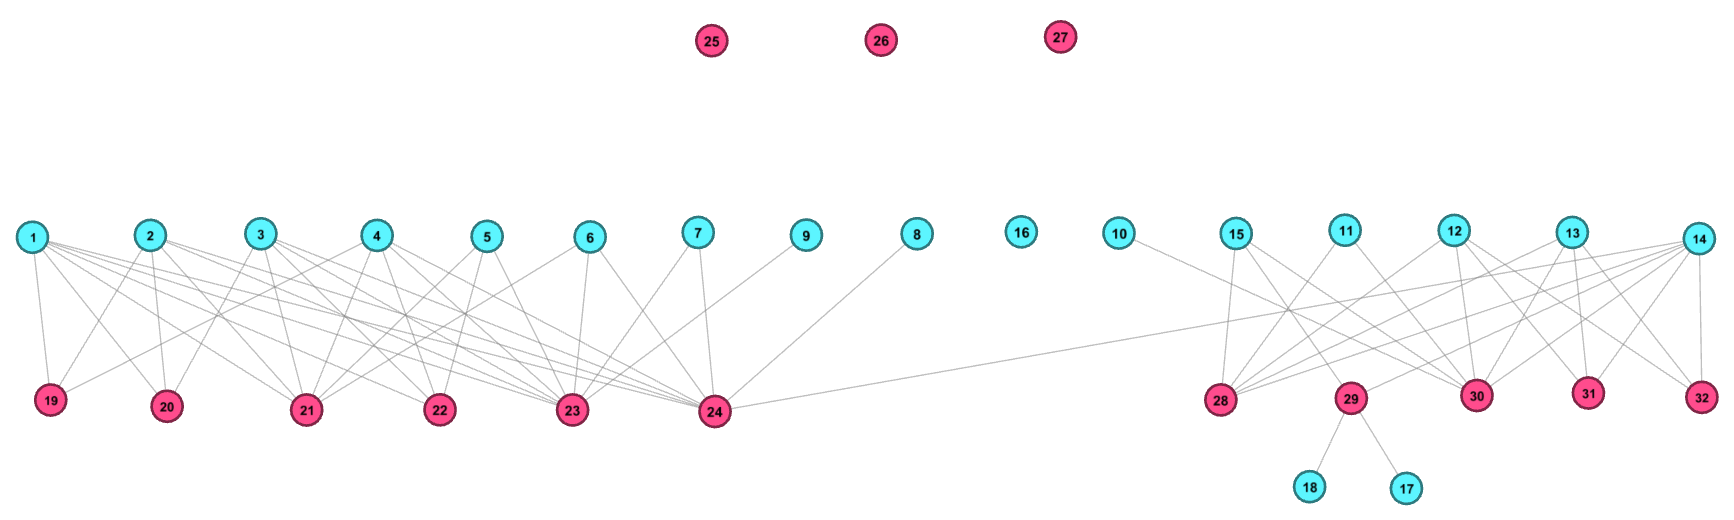
\includegraphics[width=14cm]{./figures/southern_rm.png}}
  \end{tabular}
  \caption{Southern Women dataset with \emph{tf-idf} weights and filtering
  applied}
  \label{fig:southern}
\end{figure}

The Southern women data was collected by \citet{davis1941deep} during the 1930s
and describes the participation of 18 women in 14 social events. It can be
represented as a bipartite network (figure \ref{fig:southern}) whose nodes are
women (blue nodes) and social events (red nodes). Edges are participation of the
women in the events.

This dataset and the related bipartite network was very well studied by social
scientists. Based on the ethnographic information Davis divided the 18 women
into two groups: women 1-9 in the first group, women 9-18 in the second.
Later, \citet{freeman2003finding} analyzed the outcome of 21 different
studies, which generally identified almost the same two groups, women 1-9 and
10-18. However in some of these studies women 8, 9 and 16 were often identified
as either belonging to both groups or positioned at the periphery of a group.

We applied the proposed weighting scheme to the Southern women dataset and
represented the resulted network in Figure \ref{fig:southern_tfidf}. As in the
previous example, the thickness of an edge is proportional to the \emph{tfidf}
weight. From this figure is easy to notice that edges connected to very popular
events (25, 26 and 27), where most of women participated, were assigned lower
weights than edges connected to local events (19-24 and 28-32). By applying a
threshold and removing the lower weights, two core groups of women are emerging,
as in Figure \ref{fig:southern_rm}: first group 1-9 and second 10-18. It can be
easily noticed that women 8 and 9 have a weaker connection to the first group
comparing to the other nodes in the group, while woman 16 remains isolated from
both groups.

\paragraph{Experiments}

\begin{figure}[t] \centering
  \begin{tabular}{cc} 
  \subfloat[Lastfm]{\label{fig:lastfm_cmp_edges}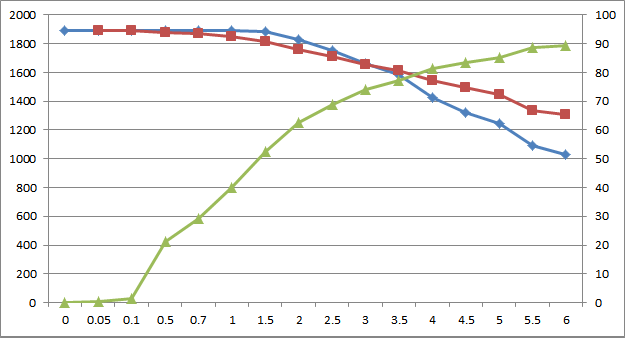
\includegraphics[width=6cm]{./figures/lastfm_cmp_edges.png}}
  &
  \subfloat[Twitter]{\label{fig:twitter_cmp_edges}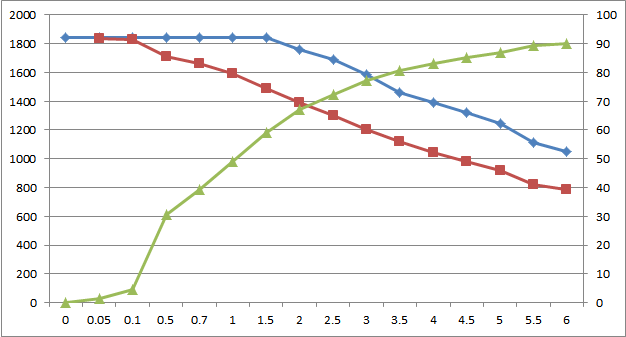
\includegraphics[width=6cm]{./figures/twitter_cmp_edges.png}}
  \\
  \subfloat[Audioscrobbler]{\label{fig:audioscrobbler_cmp_edges}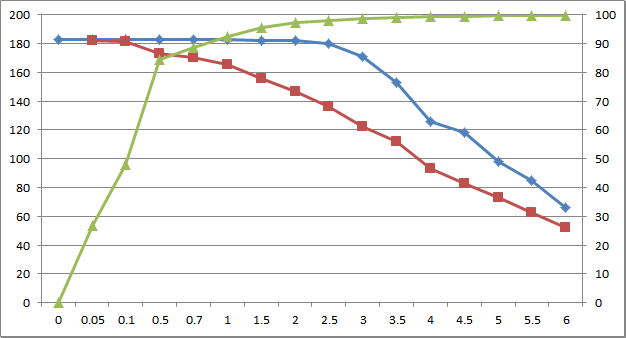
\includegraphics[width=6cm]{./figures/audioscrobbler_cmp_edges.png}}
  &
  \subfloat[Movielens]{\label{fig:movielens_cmp_edges}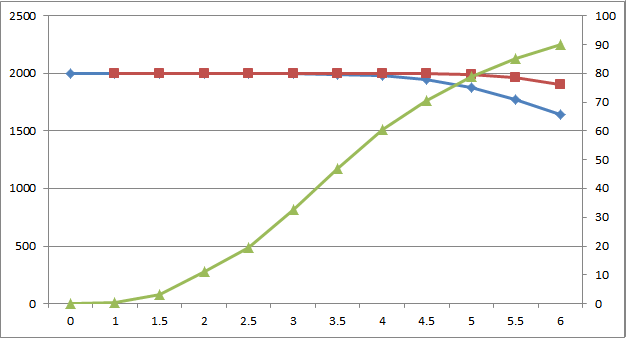
\includegraphics[width=6cm]{./figures/movielens_cmp_edges.png}}
  \end{tabular}
  \begin{tabular}{c} 
  \subfloat[Delicious]{\label{fig:delicious_cmp_edges}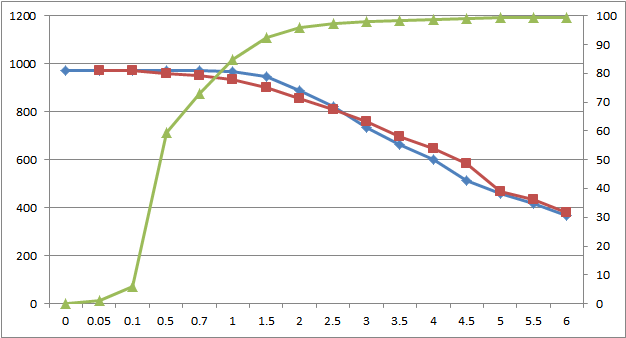
\includegraphics[width=6cm]{./figures/delicious_cmp_edges.png}}
  \end{tabular}
  \caption{Ratio of edges (green-triangle) deleted for each threshold and number
  of users in the resulted real (blue-diamond) and random (red-square) networks}
  \label{fig:cmp_edges}
\end{figure}

Next we apply the following method to each of the real world datasets. We
(re)assign the weights of edges based on the \emph{tf-idf} formula as in
equation \ref{formula:weight} and define a range of thresholds $\tau \in \{0.1,
0.5, 1, 1.5, \ldots, 6\}$. For each value $\tau$ a new network $G^{\tau} =
(U^{\tau}, O^{\tau}, E^{\tau})$ is generated by removing the edges with
\emph{tfidf} weights less than the threshold. Remaining nodes with no edges are
removed as well. We project the resulted network on user-nodes ($G^{\tau}_O$)
and apply the Louvain method for community detection \citep{blondel2008fast} in
the projection. The modularity values of the resulted partition will show the
quality of the community structure \citep{newman2004finding}.

In order to demonstrate that the proposed weighting scheme for user-object
networks improves the quality of clustering in the projections while reducing
significantly their density, for each threshold value we generate 100 similar
networks with the same number of edges removed randomly. The resulted random
networks will have the same size (nodes and edges) as the one resulted after
applying the threshold, but instead of deleting edges with \emph{tf-idf} weights
smaller than a threshold we remove them at random. We apply the same community
detection method on projections of each of these networks and compare the
average modularity across all randomly generated networks (random modularity)
with the value resulted from the network where a threshold was applied. If the
random modularity is smaller than the real value then the proposed method
improves quality of the community structure in the projected networks.

In figure \ref{fig:cmp_edges} we represent the percentage of edges removed after
applying each threshold value as above along with the number of users remaining
in both real and random networks. The number of users for random networks was
averaged for all 100 generated instances. It is quite obvious from this figure
that up to a certain threshold value (which depends on the network) the number
of user nodes remains (almost) the same after filtering is applied, even though
a significant number of edges were removed. However, in most randomly generated
networks the number of user nodes decrease at a steeper rate with the threshold.
This observation is particularly visible in Twitter and Audioscrobbler networks
where. after deleting 59\% (threshold 1.5) and 97\% (threshold 2) respectively
of edges, the number of user nodes remains the same. In the meantime, in random
case in both networks there are around 20\% less user nodes at the same
threshold values. Therefore, by applying the proposed method and filtering out
edges up to a threshold value we are preserving the same number of user nodes
(assuming a limit for the threshold), while significantly reducing the number of
edges. The resulted network will have a lower density and a more clear
structure, reflecting users most important interests.

\begin{figure}[t] \centering
  \begin{tabular}{cc} 
  \subfloat[Lastfm]{\label{fig:lastfm_cmp_density_users}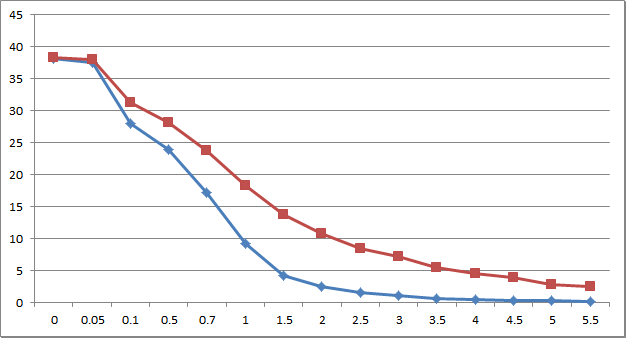
\includegraphics[width=6cm]{./figures/lastfm_cmp_density_users.png}}
  &
  \subfloat[Twitter]{\label{fig:twitter_cmp_density_users}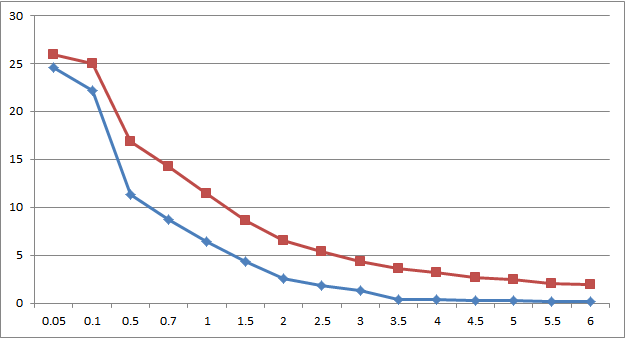
\includegraphics[width=6cm]{./figures/twitter_cmp_density_users.png}}
  \\
  \subfloat[Audioscrobbler]{\label{fig:audioscrobbler_cmp_density_users}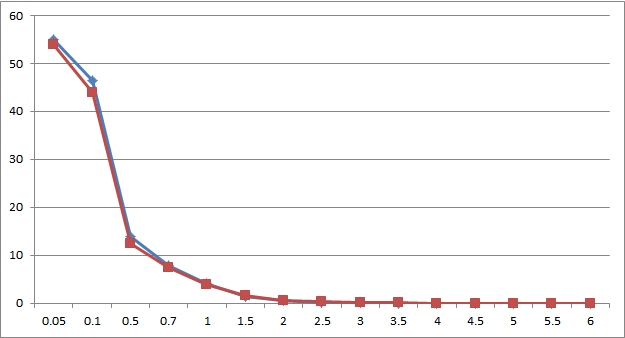
\includegraphics[width=6cm]{./figures/audioscrobbler_cmp_density_users.png}}
  &
  \subfloat[Movielens]{\label{fig:movielens_cmp_density_users}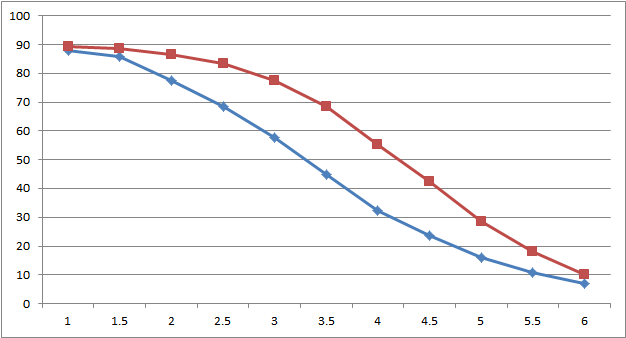
\includegraphics[width=6cm]{./figures/movielens_cmp_density_users.png}}
  \end{tabular}
  \begin{tabular}{c} 
  \subfloat[Delicious]{\label{fig:delicious_cmp_density_users}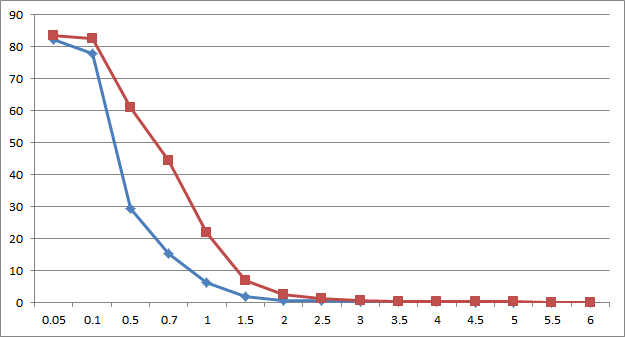
\includegraphics[width=6cm]{./figures/delicious_cmp_density_users.png}}
  \end{tabular}
  \caption{Density of user-projected network, real (blue-diamond) and random
  (red-square)}
  \label{fig:density_cmp}
\end{figure}

Next we calculate the density of the user-projected networks resulted by
applying the \emph{tfidf} weighting scheme with threshold filtering to the
original network and projecting it on the user nodes (user-projected network).
Both real and random (edges removed randomly) cases are considered for multiple
values of the threshold between 0 and 6. As above, the random density is
averaged for all 100 generated instances. As shown in figure
\ref{fig:density_cmp}, density in real networks is smaller than random networks,
for all datasets. This difference is particularly visible in Lasfm, Twitter,
Movielens and Delicious datasets, where, for some threshold values, density can
be up to 60\% less comparing to random. If we get the Twitter network for
example and select a threshold of 1.5 (no user nodes are removed by filtering)
the density of the user-projected network is 4.3, 82\% less than the original
projected network before filtering (24.6) and 50\% less than the averaged
density for random network (8.67).

\begin{figure}[t] \centering
  \begin{tabular}{cc} 
  \subfloat[Lastfm]{\label{fig:lastfm_cmp_mod_users}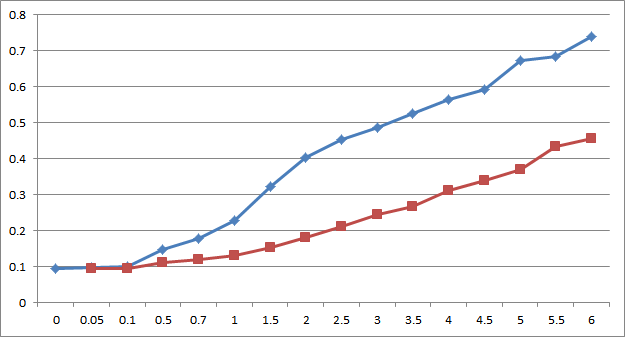
\includegraphics[width=6cm]{./figures/lastfm_cmp_mod_users.png}}
  &
  \subfloat[Twitter]{\label{fig:twitter_cmp_mod_users}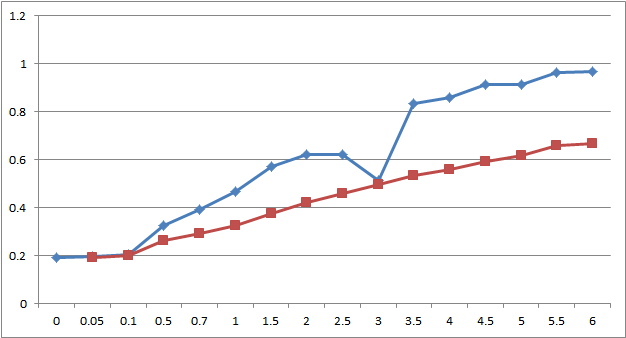
\includegraphics[width=6cm]{./figures/twitter_cmp_mod_users.png}}
  \\
  \subfloat[Audioscrobbler]{\label{fig:audioscrobbler_cmp_mod_users}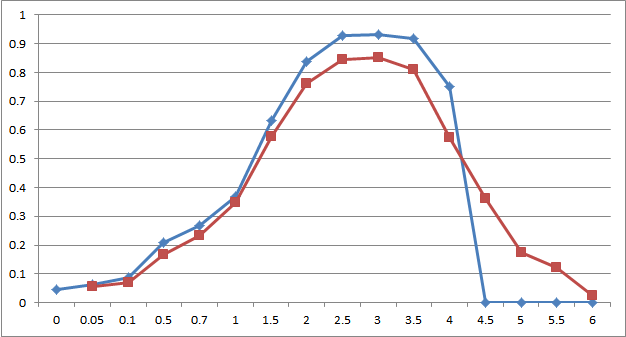
\includegraphics[width=6cm]{./figures/audioscrobbler_cmp_mod_users.png}}
  &
  \subfloat[Movielens]{\label{fig:movielens_cmp_mod_users}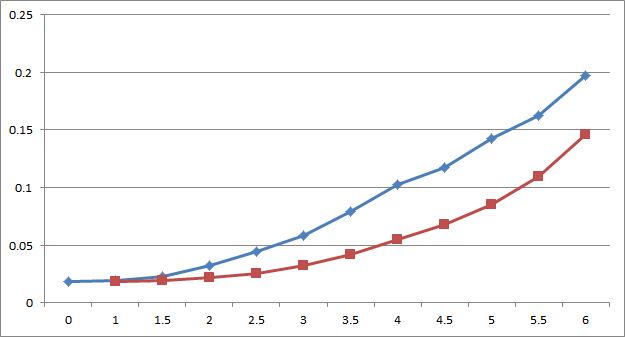
\includegraphics[width=6cm]{./figures/movielens_cmp_mod_users.png}}
  \end{tabular}
  \begin{tabular}{c} 
  \subfloat[Delicious]{\label{fig:delicious_cmp_mod_users}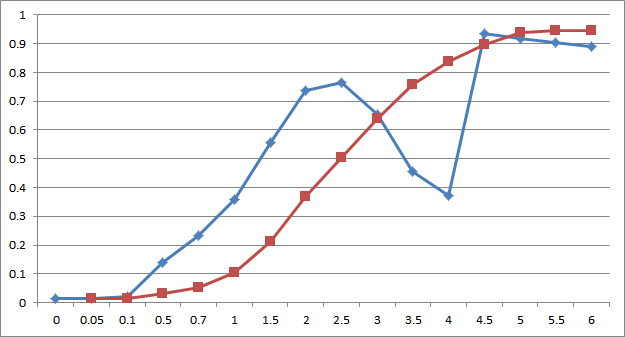
\includegraphics[width=6cm]{./figures/delicious_cmp_mod_users.png}}
  \end{tabular}
  \caption{Modularity values for partitions of user-projected network, real
  (blue-diamond) and random (red-square)}
  \label{fig:mod_cmp}
\end{figure}

Finally, after applying Louvain method for community detection on the
user-projected networks, we calculate the modularity of the resulted
partitions and compare the values for real and randomly generated networks (the
latter averaged over the 100 random instances). These values, for multiple
thresholds, are represented in figure \ref{fig:mod_cmp}. It's easy to notice
that, up to a certain threshold, modularity is constantly increasing when
higher threshold values are used and more edges are filtered out. Also, when
compared to random networks, modularity is higher with \emph{tfidf}
weighting scheme. For some datasets (Audioscrobbler and Delicious) there is a
threshold limit up to which one can notice an improvement of the proposed scheme
over the random case, but this limit is quite high in both cases. On the
other side, for Lastfm, Twitter and Movielens the difference between
real and random modularities is significantly higher. For example, taking the
same threshold value for Twitter dataset as above (1.5), the random modularity
is 34\% lower than the modularity for the real projected network. Similarly, in
Lastfm dataset random modularity is up to 54\% lower (theshold 2) comparing to
its value for the real network.

From above we saw that applying the proposed \emph{tfidf} method and filtering
out edges below a certain threshold is significantly improving both the density
of the bipartite and user-projected networks and the quality of the community
structure of the user-projected network as measured by modularity. This
improvement is also visibly better than filtering out edges randomly without
using the \emph{tfidf} weights. Therefore the resulted network has a simpler and
more intuitive structure, containing only edges that are relevant in finding
groups of similar users.
